%TODO mehr Randinfos, LEP bild, Beschreibungen
\begin{frame}
\frametitle{\secname}
\begin{timeline}{1965}{2018}{2cm}{2.5cm}{8cm}{6cm}
	\entry{1968}{Theorie: Elektroschwache Wechselwirkung}
	\pause\entry{1973}{Indirekter Nachweis durch neutrale Ströme}
	\pause\entry{1983}{Direkter Nachweis}
	\pause\entry{1989}{Präzisionsmessungen am LEP}
	\pause\entry{2012}{Nachweis des Higgs-Bosons am CERN}
	\onslide<1->
\end{timeline}
%\iffalse
\only<1> {
	\begin{textblock*}{5cm}(6.5cm,3cm) % {block width} (coords)
	\begin{figure}
		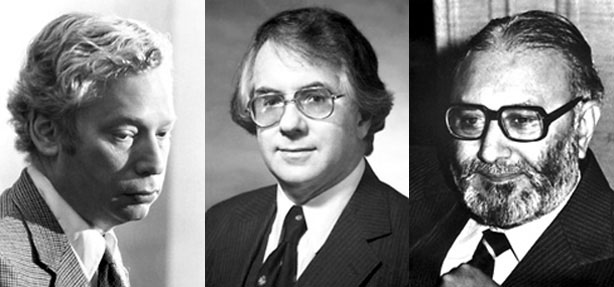
\includegraphics[width=4cm]{img/weinberg_glasgow_salam}
		\caption*{1979 Nobelpreis an Steven Weinberg, Sheldon Glashow und Abdus Salam \cite{GSW}}
	\end{figure}
\end{textblock*}
}
\iffalse
\only<2> {
	\begin{textblock*}{3.6cm}(4.5cm,3.10cm) % {block width} (coords)
	\begin{figure}
		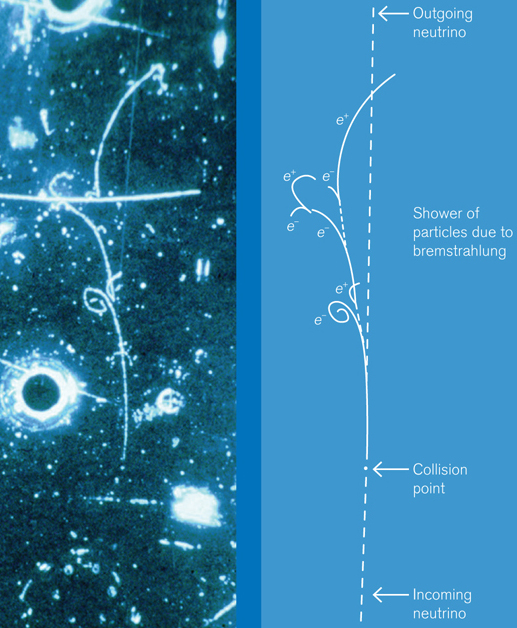
\includegraphics[width=3.6cm,angle=-90]{img/neutralerstrom}
		\caption*{Blasenkammer: $\bar{\nu}_\mu + e^- \rightarrow \bar{\nu}_\mu + e^-$ \cite{HASERT1973121}}
	\end{figure}
\end{textblock*}
}
\fi
\only<3> {
	\begin{textblock*}{3.5cm}(8cm,4.2cm) % {block width} (coords)
	\begin{figure}
		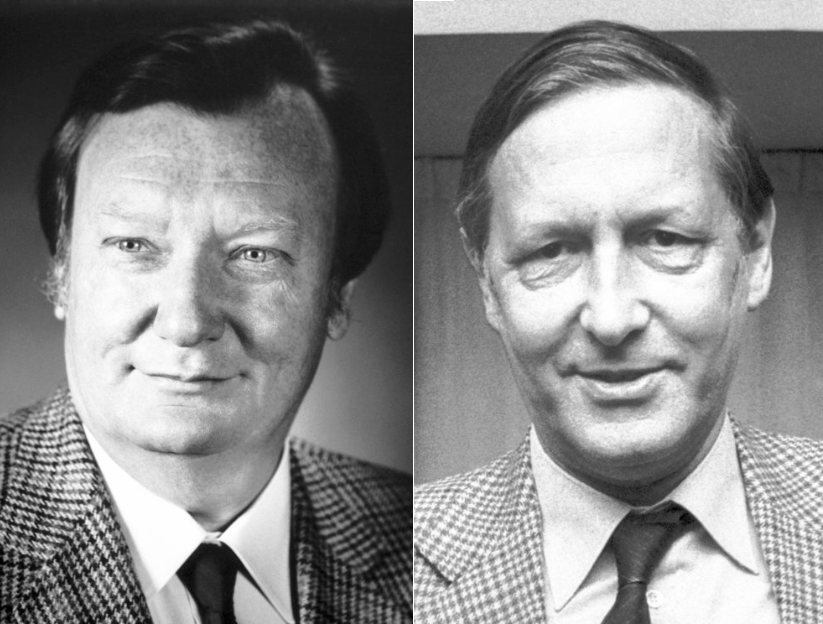
\includegraphics[width=3.5cm]{img/rubbiameer}
		\caption*{1984 Nobelpreis an Carlo Rubbia und Simon van der Meer \cite{nobel}}
	\end{figure}
\end{textblock*}
}
\only<1>{
\note[item] {Vereinheitlichung von elektr.magn. + schwache WW. Kräfteaustausch durch Photon,$W^\pm$, $Z^0$}
\note[item]{1979 Nobelpreis für GWS}
}
\only<2> {
\note[item]{Gargamelle-Blasenkammer am CERN}
}
\only<3> {
\note[item] {Am Large Electron Positorn Collider, fokus}
	\note[item]{Nobelpreis für Carlo Rubbia and Simon van der Meer für experimentelle Beitrag Proton-Antiproton-Kollisionen} %TODO Bild?
\note[item] {Mehr später}

\note[item]{Weil führte mit zum Nachweis der Z und W Bosonen}
}
\only<4> {
\note[item]{Large Electron Positron Ring (CERN) Präzessionsmessungen }
\note[item]{weiter Bestätigung der Theorie/Standardmodell und W-Z-Bosonen}
\note[item]{bis 2000}
}
\only<5> {
\note[item]{Higgs Theorie in 60er-Jahren}
\note[item]{2013 Francois Englert und Peter Higgs Nobelpreis}
\note[item]{Alle Nachweise am CERN!}
\note[item]{Randnotitz}
}
\end{frame}
